\documentclass{article} % For LaTeX2e
\usepackage{nips14submit_e,times}
\usepackage{hyperref}
\usepackage{url}
\usepackage{graphicx}
\usepackage[super]{nth}
\usepackage{todonotes}
\usepackage{amsfonts}
\usepackage[utf8]{inputenc}
\usepackage[english]{babel}

\newtheorem{theorem}{Theorem}
\newtheorem{corollary}{Corollary}[theorem]
\newtheorem{lemma}[theorem]{Lemma}

%\documentstyle[nips14submit_09,times,art10]{article} % For LaTeX 2.09

\title{CPSC 536N Project: Gossip Protocols with Random Linear Network Coding}
\author{
Neil~Newman\\
81435142\\
Department of Computer Science\\
University of British Columbia\\
\texttt{newmanne@cs.ubc.ca}
}
\newcommand{\fix}{\marginpar{FIX}}
\newcommand{\new}{\marginpar{NEW}}

\def\numNodes{\textit{n}\,}
\def\graph{\textit{G(t)}\,}
\def\graphtime{\textit{t}\,}
\def\numMessages{\textit{k}\,}
\def\RLNC{\textit{RLNC}\,}
\def\fieldSize{\textit{q}\,}
\def\dualSpace{$Y_u^{\perp}$\,}
\def\field{\mathbb{F}_{\fieldSize}\,}


\nipsfinalcopy 

\begin{document}

\maketitle

\section{Introduction}
\subsection{Gossip Protocols}
Gossip protocols are randomized algorithms used to spread information within a network. Initially, some set of messages are scattered throughout the network (each node may know none, some, or all of the messages), and the goal is to make every node in the network know all of the messages. Gossip protocols are modeled on the way that rumours spread among a society or the way in which a disease outbreak spreads throughout a population (gossip protocols are sometimes referred to as epidemic algorithms). The protocol operates through a series of rounds in which nodes exchange messages in random pairwise interactions. The message that a node chooses to send is never conditioned on who the receiver will be: the sender does not know what the receiver does or does not know.

\subsection{Why Gossip Protocols?}
Like many other randomized algorithms, gossip protocols are very simple to implement. It is also simple to reason about the eventual correctness of gossip protocols: as long as the algorithm keeps running, and as long as the graph is occasionally connected, eventually every node will hear every message. Gossip protocols are useful when it would be too expensive to send all of the information a node knows to another node at one time (for example, if the messages are database updates), or to query what the other node does or does not know. In spite of their simplicity, gossip protocols are well suited to a wide variety of network types, including dynamic networks, very large networks, and unreliable networks. In contrast to some non-randomized algorithms used to spread information through a network (for example, anything that would require constructing a spanning tree) gossip algorithms do not take the structure of the network into account. This fact makes gossip protocols suitable for use in real networks, in which communication links can fail, and nodes can enter and leave the network at any time. 

\subsection{Random Linear Network Coding}
One issue with gossip protocols is that if the goal is to spread multiple messages in parallel, a node needs to choose which information it sends in each interaction without knowledge of what the other node knows or does not know. If the node were to simply choose a random message that it knew about, it is possible for some messages to become widely spread while others remain rare, so that the stopping time for the algorithm, (the point at which every node knows all of the messages) could be dominated by the time it takes to propagate the rare messages. This can be circumvented by using gossip protocol based on \emph{Random Linear Network Coding} (RLNC). In this protocol, discussed in more detail in section \ref{subsec:RLNC}, a node sends a message that is a random linear combination of the messages that it knows, along with the corresponding coefficients. The original messages can be recovered using Gaussian elimination once a node has received enough linearly independent coefficient vectors--however, it should be noted that until this time, it is possible that the node will not be able to decode any of the individual messages (i.e. it can be all or nothing). The additional overhead of the coefficients on the packets sent is quite low if the messages are long relative to the number of messages being exchanged.

\subsection{Applications}
Gossip protocols can be applied to database replication as demonstrated in \cite{demers1987epidemic}, which describes how gossip protocols were used to share updates with other database nodes at Xerox PARC. \cite{demers1987epidemic} proposes solutions to deal with practical issues such as how a node can determine when to stop gossiping, or how to retract a previously gossiped message. Cassandra \cite{lakshman2010cassandra}, a popular distributed database management system, uses a gossip protocol in which nodes share their state information and information about a few other nodes that they know about with other nodes allowing each node to quickly build up a global picture of the network without any centralization. \cite{export:67453} describes Avalanche, a bit-torrent alternative which, instead of using a complicated scheduling algorithm for thinking about what blocks to download, simply uses RLNC.

\subsection{This paper}
The goals of this paper are as follows: Firstly, to summarize the results and techniques used to prove bounds on the expected stopping times of gossip protocols based on RLNC in \cite{haeupler2011analyzing}. Secondly, to check experimentally the expected stopping times given for a specific setting, known as the Random Phone Call Model (see section \ref{subsec:randomphonecall}), of the RLNC gossip algorithm and compare with the theoretical results. 

\section{Model of Network and Communication}
We will use the model from \cite{haeupler2011analyzing}, which is as follows: There are \numNodes nodes in the network. A network is a graph \graph that can be static ($\graph = G  \forall \graphtime$) or can vary with time \graphtime and is either directed or undirected. An edge in \graph from any two nodes \textit{a} and \textit{b} represents a link through which communication can take place in round \graphtime; if the edge is directed it means that communication can only occur in the direction of the edge. There are \numMessages messages distributed over the network (see \ref{subsec:startingconditions} for details on the ways in which we consider the messages to be distributed). Each message is of fixed length $l$.

\subsection{Modes of communication}\label{subsec:communication}
We allow the following modes of communication:
\begin{itemize}
	\item \texttt{BROADCAST} A node sends to all of its neighbours
	\item \texttt{PUSH} A node sends to one neighbour chosen uniformly at random
	\item \texttt{PULL} A node chooses a neighbour uniformly at random and receives a message from that neighbour
\end{itemize}

\subsection{Starting conditions}\label{subsec:startingconditions}
We consider the following starting conditions:
\begin{itemize}
	\item \texttt{WORST CASE} A single node beings knowing every message, while other nodes know nothing
	\item \texttt{WELL MIXED} Each message is initially known by a distinct node (i.e. if $\numMessages=2$ and $\numNodes=3$ we could have node $u$ knows message 1, node $v$ knows message 2, and node $w$ knows nothing).
\end{itemize}

\section{RLNC Algorithm}\label{subsec:RLNC}
In this section we describe in detail the RLNC algorithm.
\subsection{Preliminaries}
Packets are vectors over a finite field $\mathbb{F}_{\fieldSize}$, where the size of the field, \fieldSize, is a prime or prime power. Addition and multiplication in the remainder of this description are over $\mathbb{F}_{\fieldSize}$. There are \numMessages messages, $\vec{m_{1}}...\vec{m_{\numMessages}}$ that are vectors from $\mathbb{F}_{\fieldSize}^{l}$ where $l$ is the message length. Packets are of the form ($\vec{\mu}, \vec{m}$), where $\vec{m} = \sum_{i=1}^{\numMessages} \mu_i\vec{m_i} \in \mathbb{F}_{\fieldSize}^{l}$ and $\vec{\mu} = (\mu_1,...,\mu_k) \in \mathbb{F}_{\fieldSize}^{\numMessages}$ is the coefficient vector. Note that if a node ever knows enough coefficient vectors such that the span of these vectors is $\mathbb{F}_{\fieldSize}^{\numMessages}$ then Gaussian elimination can be used to reconstruct all of the messages. Therefore, \numMessages packets with linearly independent coefficient vectors are needed in order for a node to decode all of the messages. The choice of \fieldSize is a trade-off between the size of messages in bytes (because of the space needed to store the coefficients) and the convergence rate; we use $\fieldSize=2$ for the remainder of this paper. 
\subsection{RLNC Algorithm}
Every node \textit{v} keeps a subspace $X_v$ that is the span of all of the packets it currently knows. When a node needs to choose a packet to send, it picks a packet uniformly at random from $X_v$. When a packet is received, $X_v$ is recomputed. If the coefficient vectors span the entire space, then a node can decode messages. When this is true for every node, the algorithm is considered to have stopped. At this point, every node can use Gaussian elimination to recover the original messages.
\subsection{Practical Details}
This section describes practical details about how the RLNC algorithm was implemented in our simulator. Every node maintains only messages that are \textit{helpful}, that is, messages that increase the rank of the coefficient matrix: a matrix in which every row corresponds to a previously received message's coefficients. We refer to the subspace spanned by these coefficients as $Y_v$. If a node begins knowing a particular message, say message $i$, then it's coefficient matrix is initialized to begin with the $ith$ standard basis vector. To determine whether or not a new message contains helpful coefficients, we compute both the rank of the current matrix and the rank of the current matrix with an additional row for the new message's coefficients. If the rank has increased, the message is helpful and we add it to the node's collection of messages (and its coefficients to the coefficient matrix). Otherwise, the message provided no new information, and so it is ignored. When the rank of the coefficient matrix is equal to the number of messages, a node can decode all of the messages. When this condition is true for every node, we say that the algorithm has terminated. In order to send out a random message, a node generates a uniformly random coefficient in $\mathbb{F}_{\fieldSize}$ for each message it knows, and then sends out the linear combination of its known messages and the corresponding coefficients.

\section{Proof techniques and summary of theoretical results}
\subsection{Perfect Pipelining}
If an algorithm achieves a stopping time of $O(\numMessages + T)$, where $T$ is the time that it takes to distribute a single message amongst all of the nodes, then it is said to achieve perfect pipelining. In perfect pipelining, the startup cost is paid only once, and every subsequent message does not need to pay for the time to cross the graph. 

\subsection{General analysis technique}
In order to determine the expected stopping times for gossip RLNC protocols, \cite{haeupler2011analyzing} looks at how the orthogonal complement of the coefficient space $Y_u$, \dualSpace, shrinks monotonically to the empty span as a node learns new, linearly independent packets. Note that because we are operating in a field, the dot-product is not positive definite and so the concept of orthogonal does not match geometrical intuition.  They pick a fixed vector in \dualSpace and determine how many rounds it takes before it vanishes from $Y_u$ with high probability. Then a union bound is taken over every one of the $\fieldSize^{\numMessages}$ vectors in \dualSpace. They rely on the following definition of \textit{knowing} a vector throughout the paper:
\begin{lemma}
A node knows about $\vec{\mu} \in \field$ if its coefficient subspace $Y_u$ is not orthogonal to $\vec{\mu}$ ($\exists \vec{c} \in Y_u s.t. <\vec{c},\vec{\mu}>\neq0$). If a node $u$ knows about $\vec{\mu}$ and sends a packet to node $v$, then node $v$ knows $\vec{\mu}$ afterwards with probability at least $1-1/\fieldSize$. If a node knows all vectors in $\mathbb{F}_{\fieldSize}^{\numMessages}$, then it can decode all the messages.
\end{lemma}

The $1-1/\fieldSize$ result comes from that fact that vectors in $Y_u$ that are perpendicular to $\vec{\mu}$ form a hyperplane in $Y_u$. Knowledge about a particular $\vec{\mu}$ spreads with probability $1-1/\fieldSize$. The spread of knowledge of a fixed vector over all of the nodes is a monotone increasing set growing process. It can be modeled as a monotone Markov process and therefore the time to spread the knowledge to all nodes has an exponentially decaying tail. The paper uses the following theorem to relate results for gossip protocols to gossip protocols based on RLNC. 
\begin{theorem}\label{theorem:template}
Choose a $\delta > 0$. Imagine that in some \graph with a fixed communication mode (see section \ref{subsec:communication}), a node $v$ tries to disseminate a single message. It does this in the following way: every round, every communication that is supposed to occur according to the communication mode fails with probability $1/\fieldSize$. If, for every choice of $v$ in the network, the probability that the message is successfully spread after \graphtime rounds is at least $1-\delta\fieldSize^{-\numMessages}$, then \numMessages messages could be spread in the same network in time \graphtime with probability $1-\delta$ using RLNC gossip with a field size \fieldSize. 
\end{theorem}
The theorem works because if a node $u$ sends a message to node $v$ and $u$ knows $\vec{\mu}$, then $v$ will now know $\vec{\mu}$ with probability $1-1/\fieldSize$. This is equivalent to the faulty broadcasting system described above. We assumed that after \graphtime steps, the probability for any given vector that it failed to spread is at most $\delta\fieldSize^{-\numMessages}$, so taking a union bound over all $\fieldSize^{\numMessages}$ vectors gives a probability that after \graphtime rounds all nodes know about all vectors with probability at least $1-\delta$.

\subsection{Proof Template}\label{subsec:template}
Most proofs in the paper are based on applying theorem \ref{theorem:template}. The trick then becomes to model the time it takes to disseminate a single vector in the faulty communication model. Typically they show that the time for a single vector to spread is dominated by a negative binomial distribution, $NB(T,1-p)$ where $p$ is a constant probability and $T$ is the number of successful rounds needed to spread a single vector. The tail of this distribution is strong enough to prove $O(T+k)$ stopping times. The exact definition of a success will depend on the network properties (expansion, cuts, diameter etc.) and will determine how many nodes need to learn about the vector in a successful round. A Chernoff bound can be used to show that the probability that a a vector has not spread after $c(k+T+\log{\delta})$ steps is at most $2^{-O(k+T+\log{\delta})}$, which after a union bound over all $q^k$ vectors, means that the probability that all the messages have not spread is at most $\delta$. 

\subsection{Complete graphs - The Random Phone Call Model}\label{subsec:randomphonecall}
The random phone call model is a model where \graph is the complete graph. At each time \graphtime, every node randomly phones another node and either PUSH or PULL communication takes place.  In a complete graph, RLNC gossip achieves perfect pipelining, and $T$ is $\Theta(\log{n})$ with high probability. The proof uses the basic template described above in section \ref{subsec:template} to construct the upper bound. 
\paragraph{Lower bound}
A node has a $\frac{1}{\numNodes-1}$ chance of being dialed by another node, and since this true for all $\numNodes-1$ nodes, a node receives in expectation $\Theta(1)$ packets in a round. If even a single node does not know any messages at the start, the algorithm must run for at least $\Omega(\numMessages)$ rounds. Imagining that a single node tries to spread a single message, it will take at least $\Omega(\log{n})$ time to spread it to all nodes (in the best case, after the first round, 1 node knows the message, then 2 nodes after the second, then 4 nodes after the third etc.). Therefore, this model is $\Omega(\numMessages + \log{n})$.
\paragraph{Upper bound}
Now the template from section \ref{subsec:template} is used. To show that the random phone call model is also $O(\numMessages + \log{n})$, they fix a coefficient vector $\vec{\mu}$ and label a successful round as one in which the number of nodes that know about $\vec{\mu}$ increases by a constant factor, $\lambda > 1$. Because of this constant factor, it will take at most $O(\log{n})$ rounds until every node knows about $\vec{\mu}$. To use theorem \ref{theorem:template}, they show that a successful round occurs with constant probability. We will summarize the proof for the PULL model. At first, $i < \numNodes/2$ nodes know about $\vec{\mu}$ and therefore at least $\numNodes/2$ nodes are trying to pull $\vec{\mu}$. Each individual node will pull from a node that knows $\vec{\mu}$ with probability $i/\numNodes$, and therefore in expectation at least $i/2$ nodes will receive a message from a node that knows $\vec{\mu}$. With a fixed \fieldSize, after such a pull the node will know $\vec{\mu}$ with probability $1-1/\fieldSize$.  Therefore, at least $\Omega(i)$ nodes learn $\vec{\mu}$ with constant probability each round. After $n/2$ nodes know $\vec{\mu}$, an ignorant node can pull $\vec{\mu}$ with probability at least $1/2$.
\paragraph{Stronger result for PULL and well mixed messages}
A later result in the paper with more careful reasoning shows that in the random phone call model with the PULL type communication, $k>\log{n}^{1+o(1)}$ messages can be spread in $k(1+o(1))$ time if a each message is initially known to a unique node.

\subsection{BROADCAST in Dynamic Networks}
If a graph is static, the time it takes to broadcast a single message is the diameter of the graph, $D$, and so the time to spread \numMessages messages will be $\Theta(D + \numMessages)$. This is not true of a graph that can evolve over time. Consider an adversary that gets to choose the set of edges at every time \graphtime (subject to the constraint that \graph must remain connected). If there is only a single message to distribute, an adversary might choose to only put a single link between the set of nodes that know the message and the set of nodes that don't know the message. Then $D=2$, but it will still take at least \numNodes rounds for the message to spread. Therefore, the paper chooses to look at the isoperimetric number $h(G)$:
\begin{equation}
h(G) := \min\limits_{S \subseteq V}{\frac{|\Gamma^{+}_G(S)|}{\min{|\overline{S}|,|S|}}}
\end{equation} 
where $\Gamma^{+}_G(S)$ are nodes in $G$ outside of $S$ that are in the directed neighbourhood of $S$. This number is a rough measure of how bottlenecked a graph is. They show that the expected time to distribute one message is at most $T=\frac{\log{(nh(G))}}{h(G)}$. This leads to the result that BROADCAST can spread \numMessages messages with high probability in at most $O(\frac{\log{(nh)}}{h} + \numMessages)$ rounds as long as $h(\graph) >= h \forall \graphtime$. The proof uses the template presented in section \ref{subsec:template} by defining a successful round as one in which the number of nodes that know $\vec{\mu}$ grows by at least $\frac{h}{7}$ and then argues that at most $O(\frac{\log{nh}}{h})$ successes are needed to spread the vector completely and shows that this occurs with a constant probability. 

\subsection{Random Networks}
Many proofs rely on connectivity properties of \graph that have to hold for every time \graphtime. The paper's insight is that we can also consider the union of graphs over multiple rounds, $G'(t) = G(3t') \cup G(3t'+1) \cup G(3t'+2)$ to reason about networks in which certain connectivity properties might hold in expectation over several rounds.

\section{Experiments}
We experimented with the Random Phone Call model discussed above in section \ref{subsec:randomphonecall}. We ran simulations of RLNC gossip with interest in answering the following questions: Do the simulation results have stopping times that grow according to the theoretical results, both when we vary the number of messages \numMessages and the number of nodes \numNodes? What is the impact of PUSH vs. PULL communication? What is the impact of using RLNC as opposed to a simpler gossip algorithm? Experiments were performed using a simulator built in \textit{python} and \textit{sage}\cite{sage}. The messages were all of length $l=100$ The field size was $q=2$. 5 trials were run on every configuration.
\subsection{Comparison to Theoretical Bounds}
Figure \ref{fig:rlnc-vary-k} plots how the stopping time varies as the number of messages \numMessages is increased. The growth seems to be linear in the number of messages, as predicted in \cite{haeupler2011analyzing}. Figure \ref{fig:rlnc-vary-n} plots how the stopping time varies as the number of nodes \numNodes is increased. The graph is consistent with the logarithmic bound proven in \cite{haeupler2011analyzing}. Both figures \ref{fig:rlnc-vary-k} and \ref{fig:rlnc-vary-n} also plot the difference between using PUSH and PULL. Based on the results, it seems that the PULL model leads to a quicker stopping time when both \numMessages and \numNodes are varied. This makes sense, since for example if a single node knows a message it can only inform one other node in the PUSH model per round, however, any number of nodes that connect to this node might learn the rare message.

\subsection{Comparison to Simple Gossip}
In this section we ask what the gain of using RLNC is in terms of stopping time, as compared to using a simpler gossip protocol. In the simple protocol, nodes do not do any network coding, and simply send out a single, entire message. The results are summarized in \ref{fig:rlnc-ecdf}, which plots cumulative distributions of the stopping times, showing what fraction of the nodes can decode all of the messages at any given round. It is clear from the figure that the RLNC algorithm converges much more quickly than simple gossip. We also see again that in the simple model, PULL converges more quickly than PUSH.

\begin{figure}
	\centering
	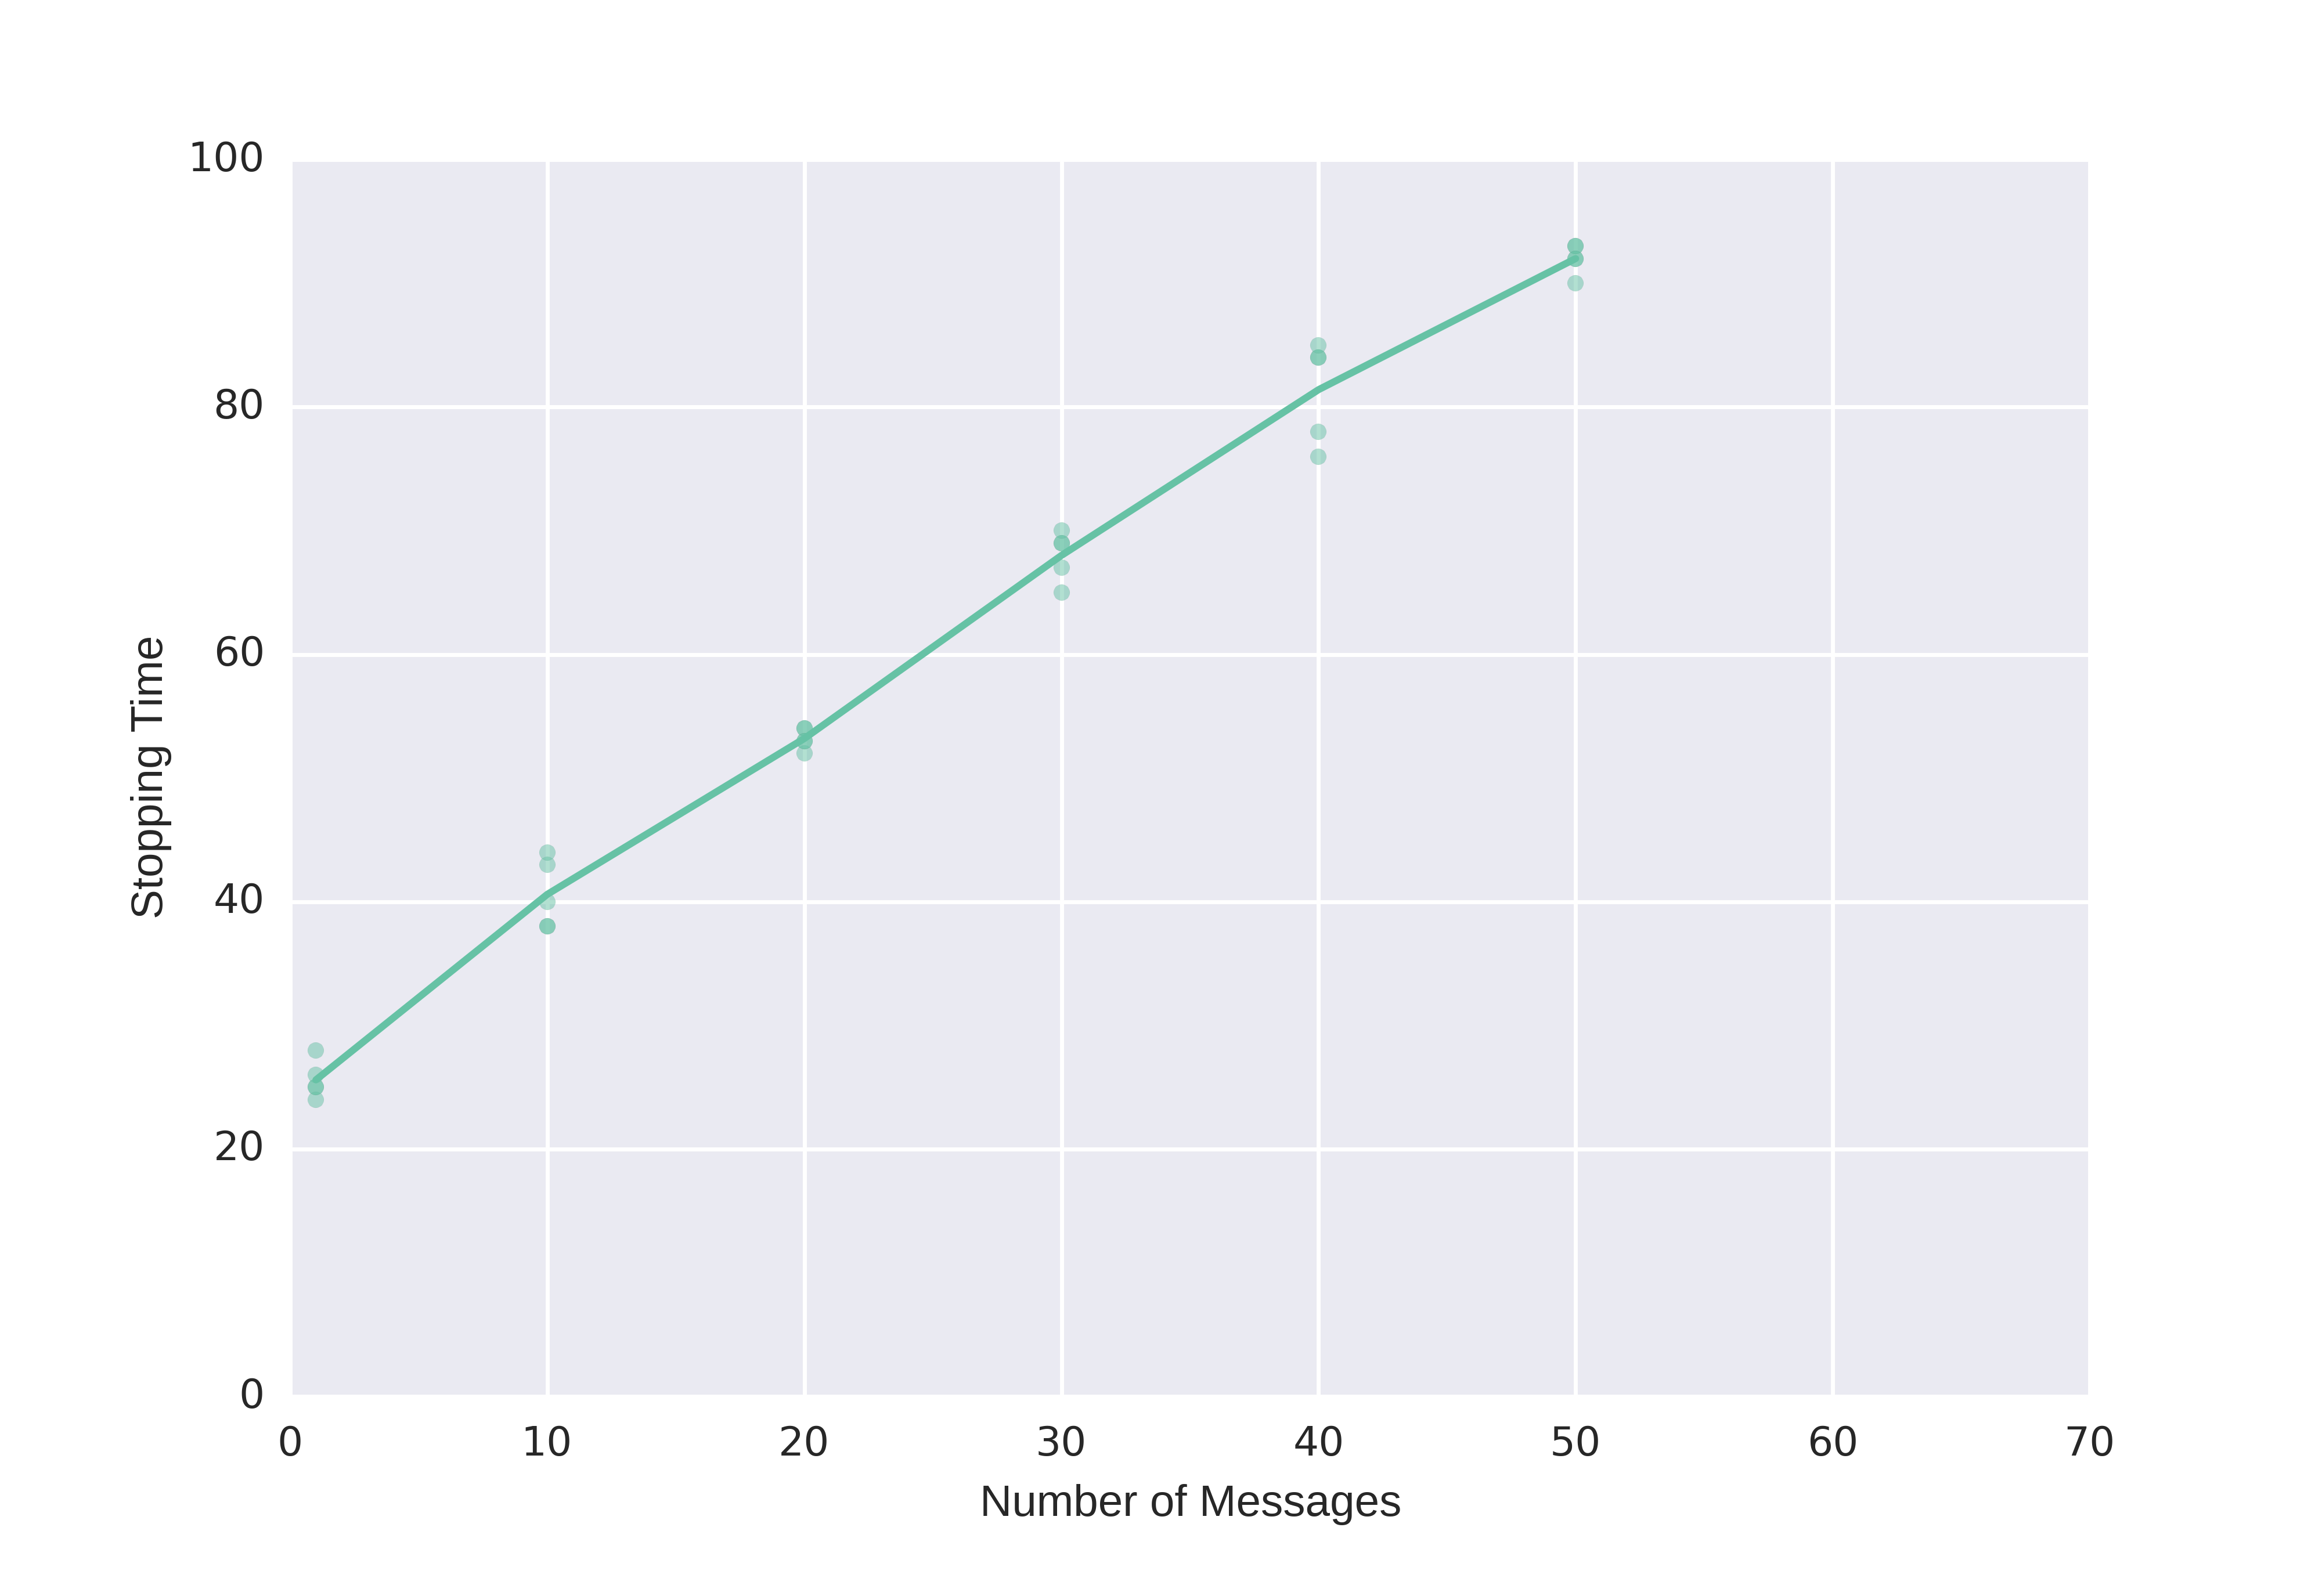
\includegraphics[width=\linewidth]{figures/rlnc-vary-k.png}
	\caption{The stopping time of RLNC Random Phone Call algorithm is plotted with both PUSH and PULL interactions as the number of messages, \numMessages, is varied. $\numNodes=500$ is fixed for all values of \numMessages. The number of rounds that it takes for the algorithm to terminate appears to be linear in the number in \numMessages, as theory predicts.}
	\label{fig:rlnc-vary-k}
\end{figure} 
\begin{figure}
	\centering
	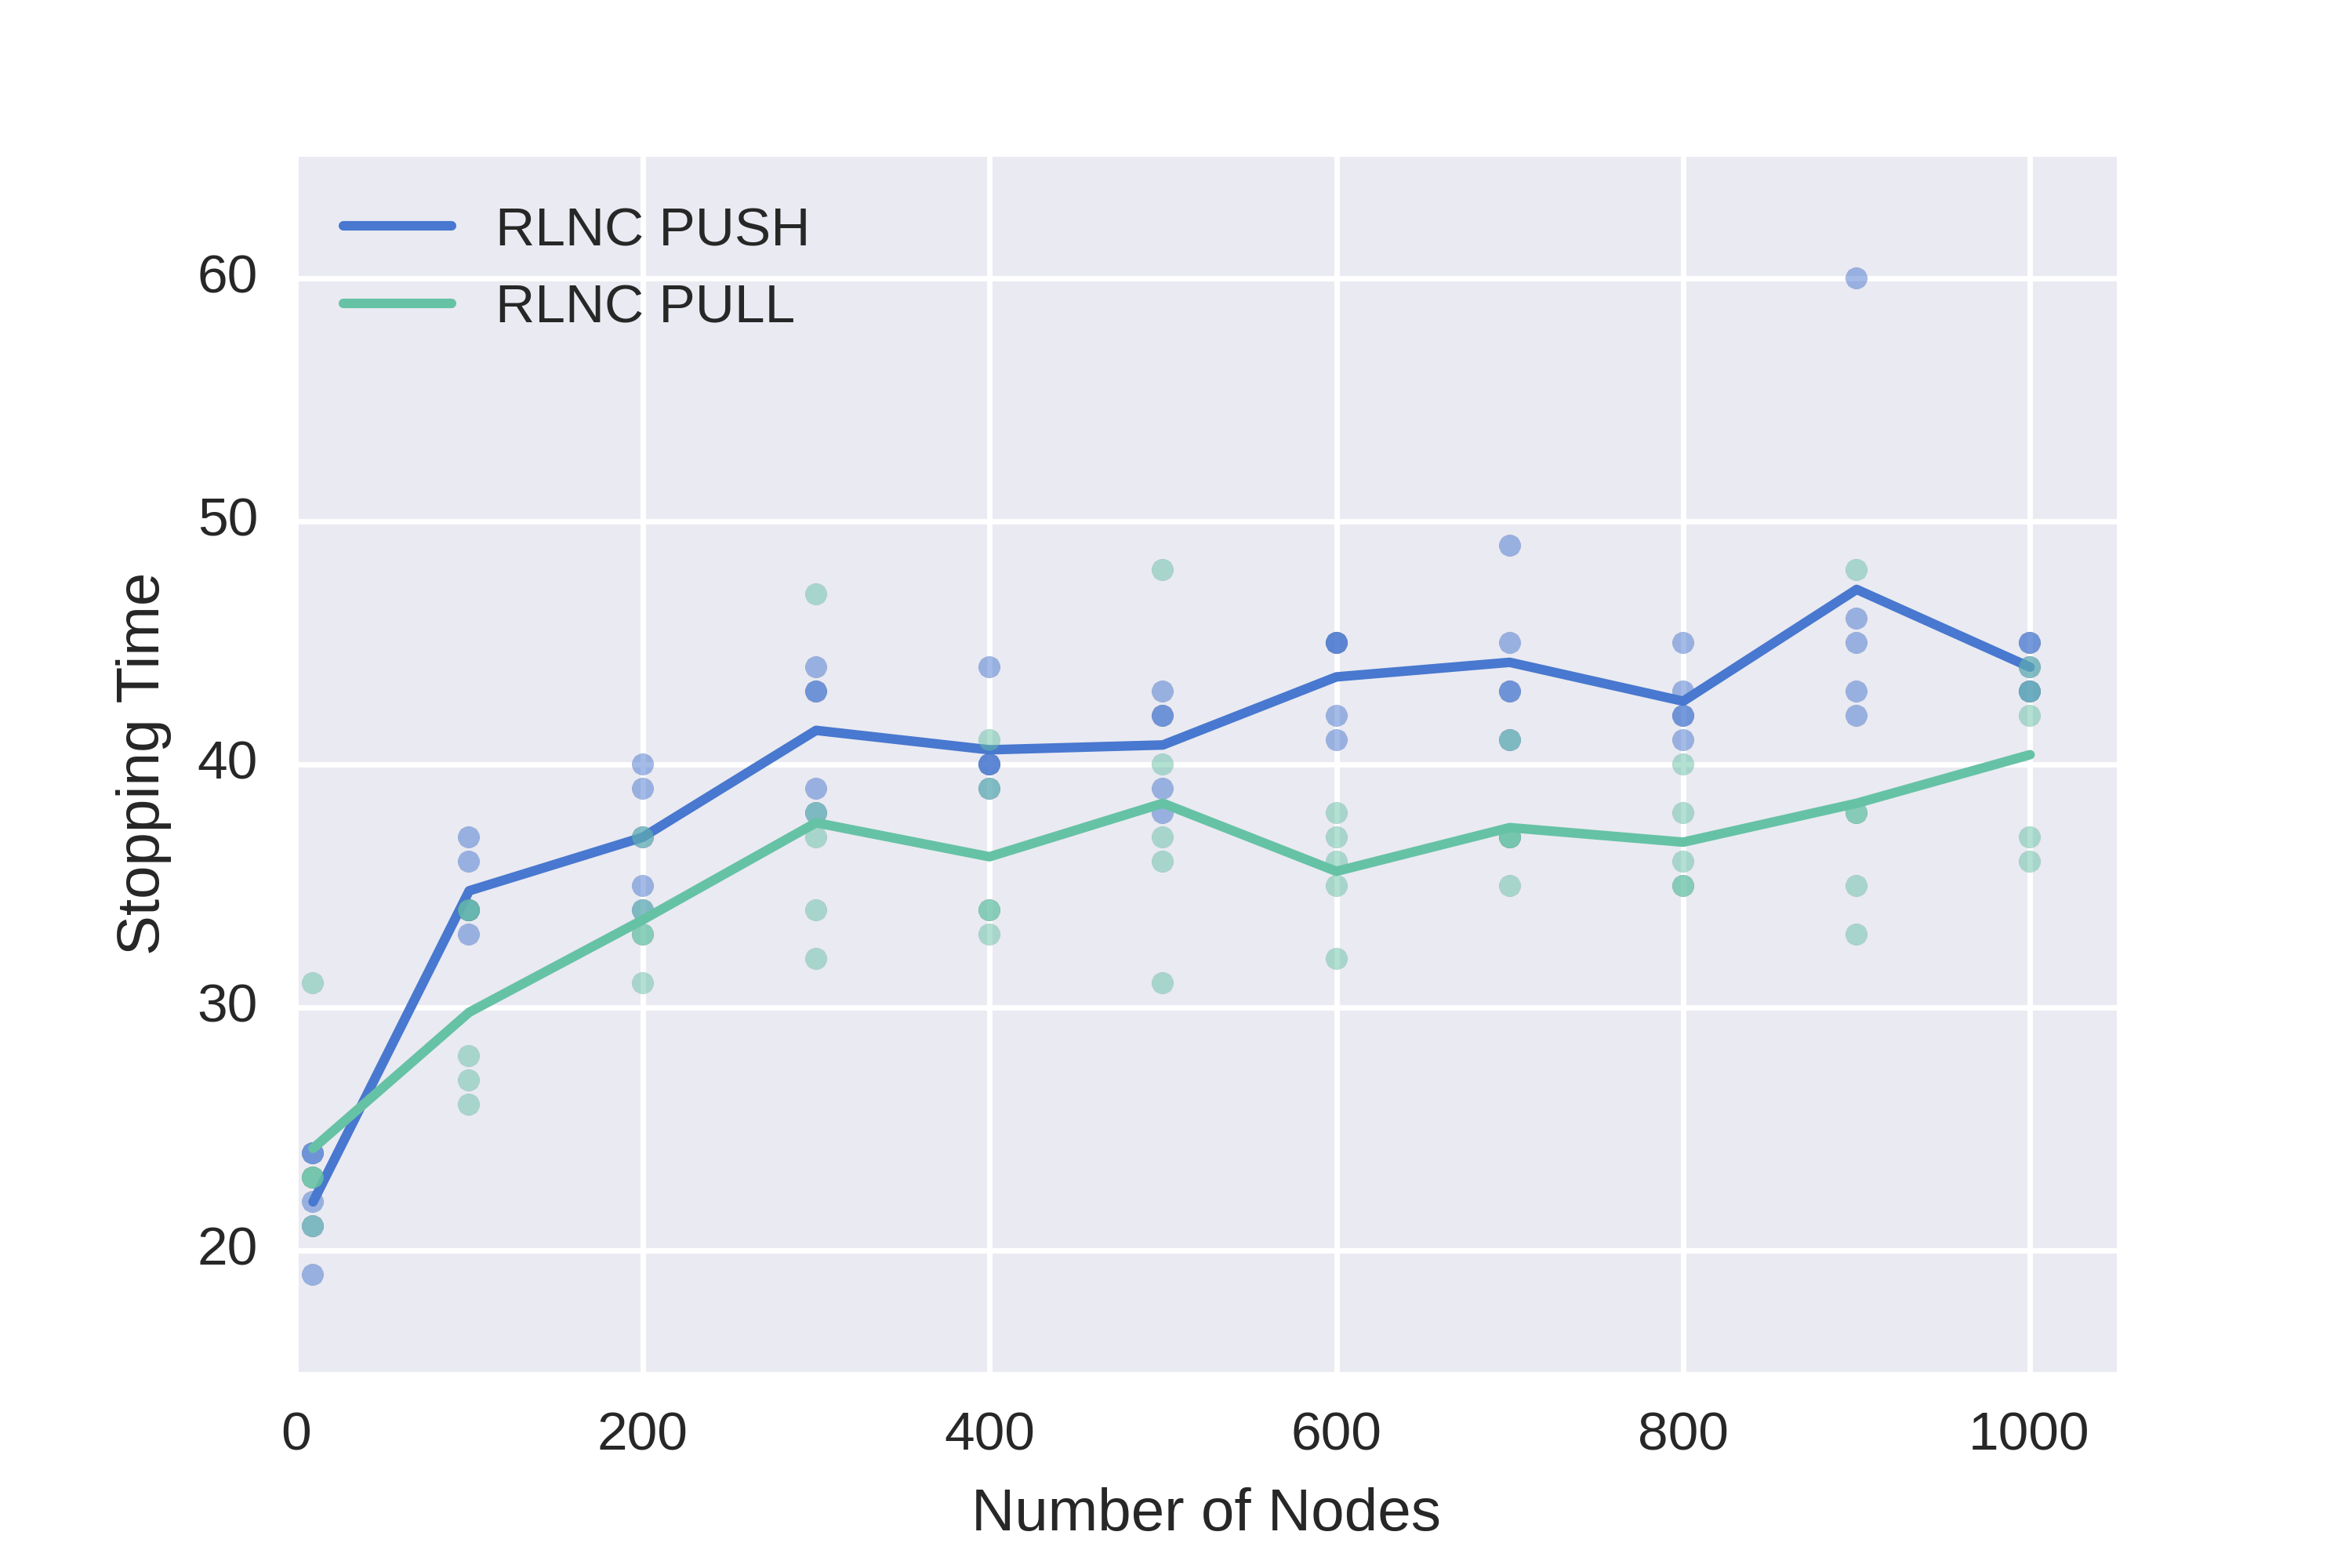
\includegraphics[width=\linewidth]{figures/rlnc-vary-n.png}
	\caption{The stopping time of the RLNC Random Phone Call algorithm is plotted with both PUSH and PULL interactions as the number of nodes, \numNodes, varied. $\numMessages=10$ is fixed for all values of \numNodes. The number of rounds that it takes for the algorithm to terminate appears to be logarithmic in \numNodes, as theory predicts.}
	\label{fig:rlnc-vary-n}
\end{figure} 
\begin{figure}
\centering
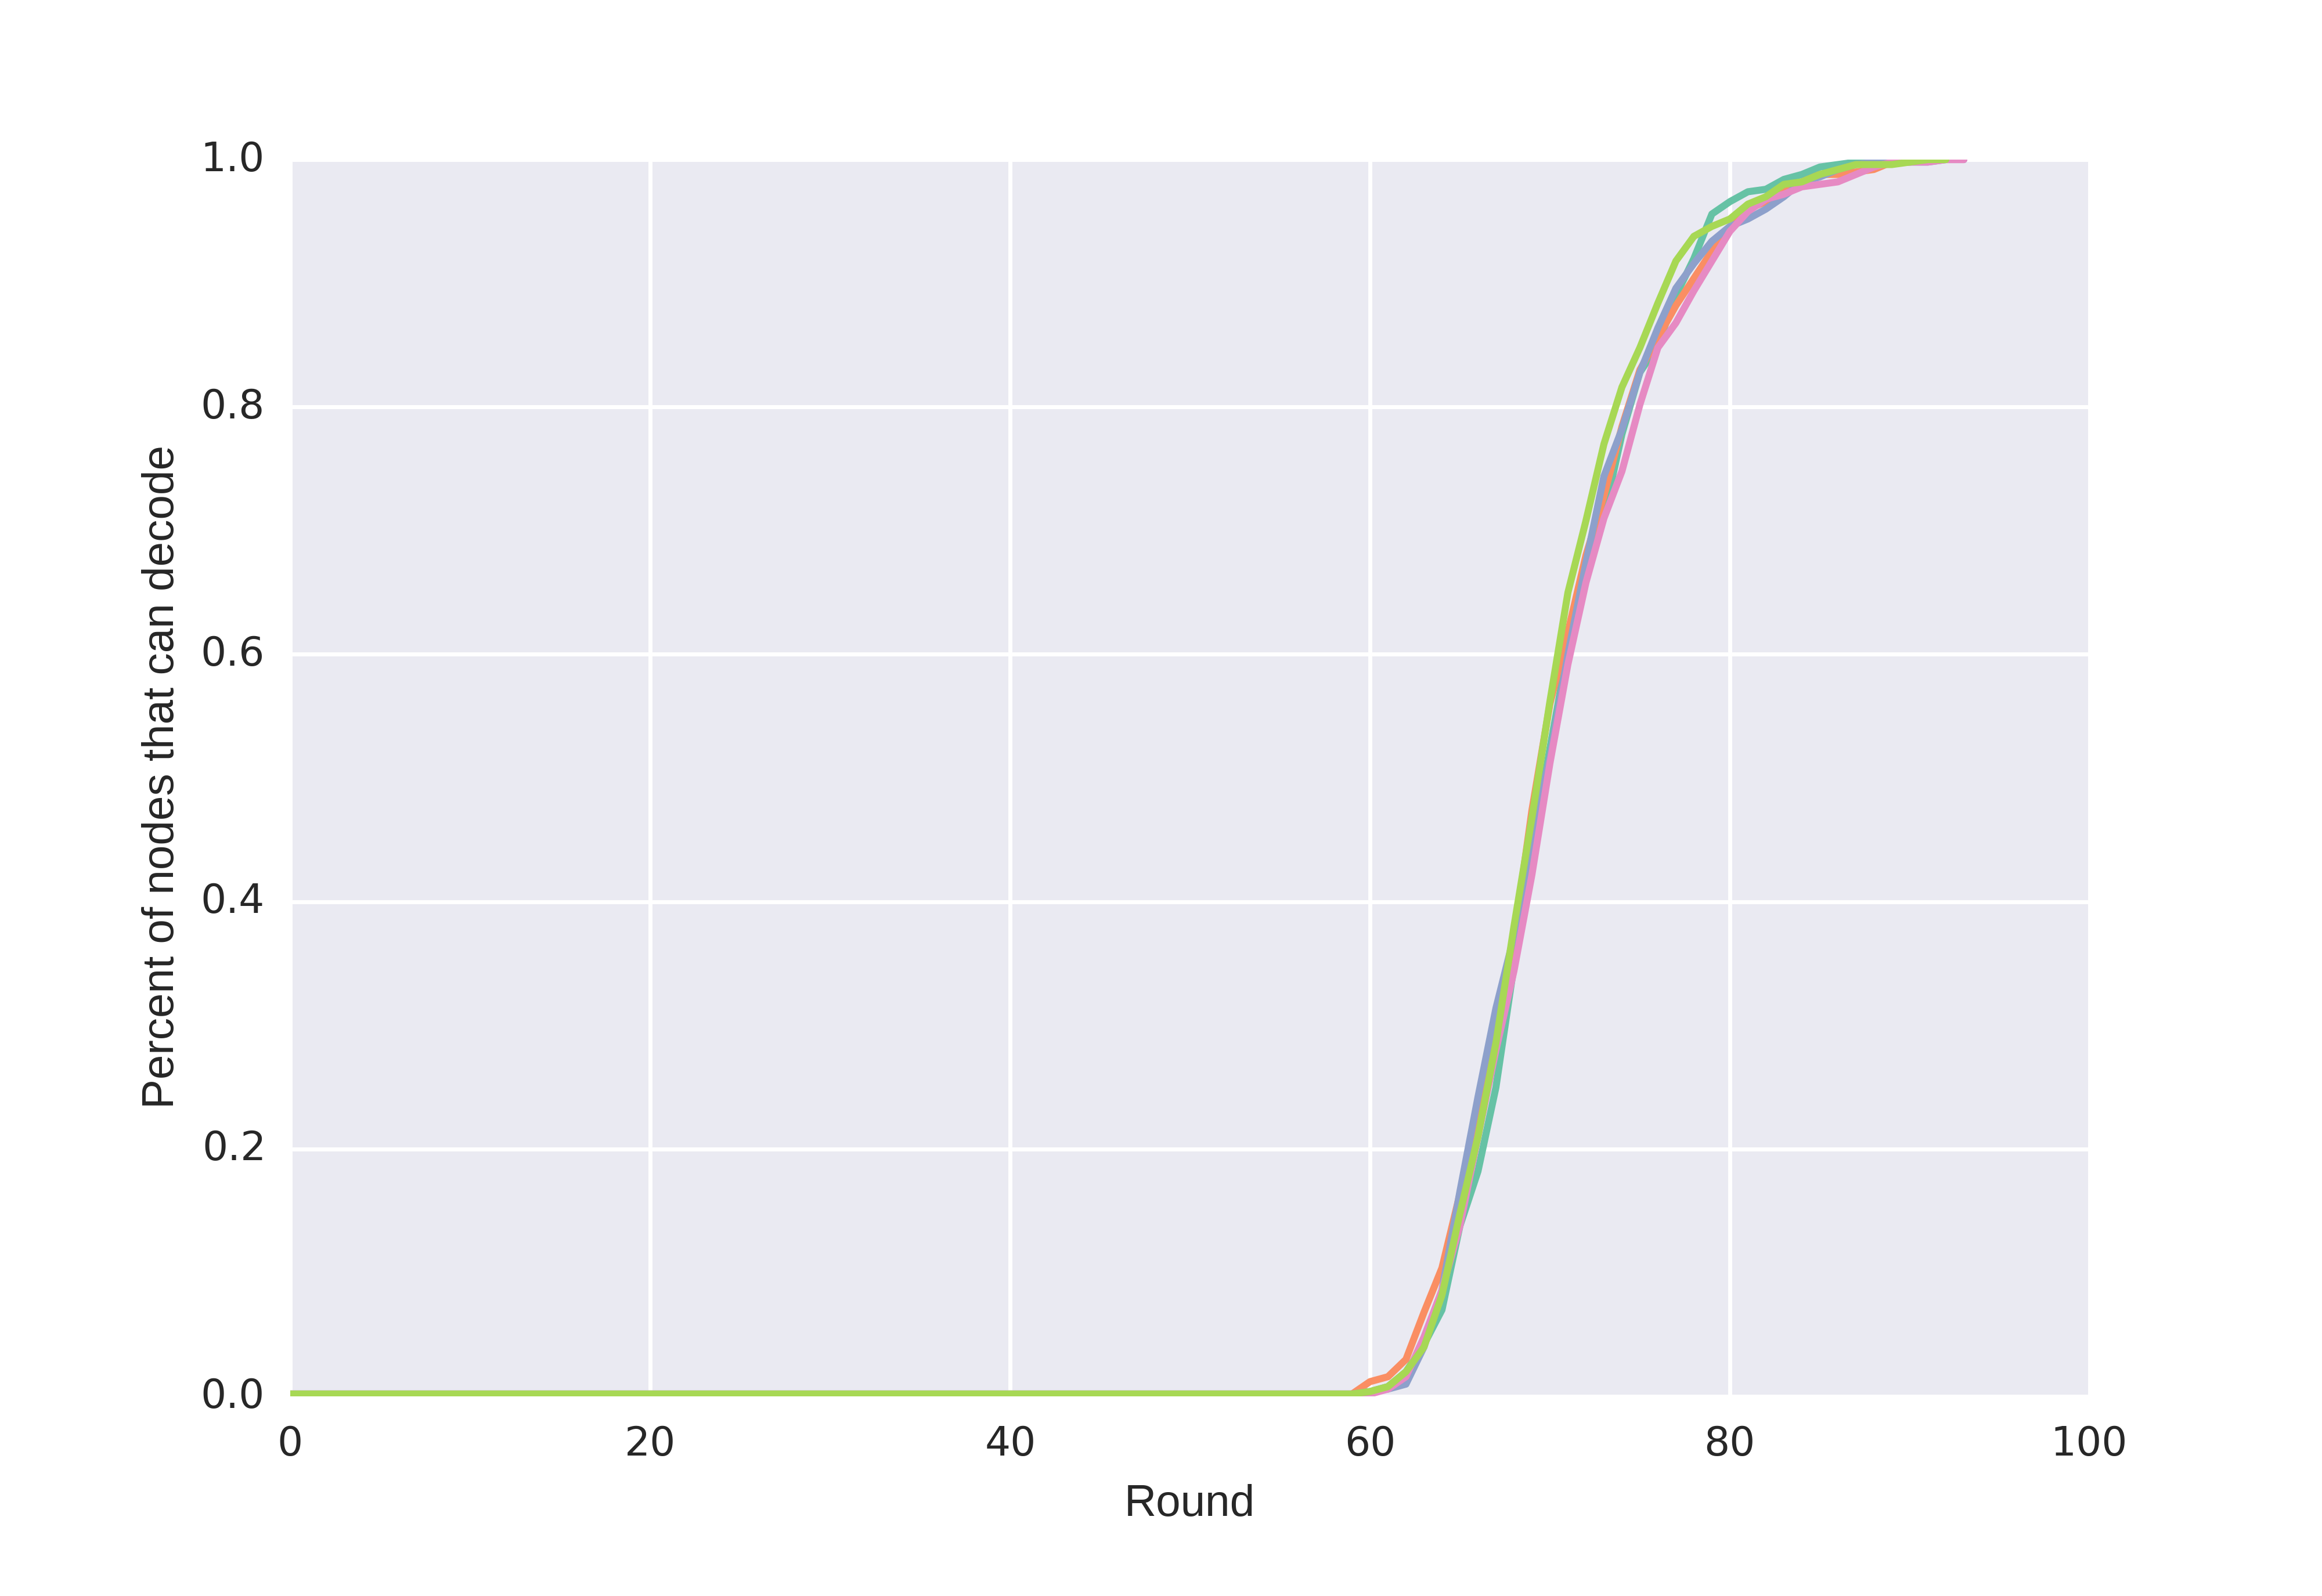
\includegraphics[width=\linewidth]{figures/ecdf.png}
\caption{Cumulative distribution showing what fraction of nodes can decode the messages at any given round. Data is taken from 5 trials in the Random Phone Call model with $\numNodes=500$ nodes and $\numMessages=50$ messages. The stopping time of RLNC is compared to the stopping time of simply sending a random message.}
\label{fig:rlnc-ecdf}
\end{figure} 

\section{Conclusions and Future Work}
We have summarized results from \cite{haeupler2011analyzing} about the time complexity of gossip protocols using RLNC. We then presented results from a series of simulations which confirmed the results in \cite{haeupler2011analyzing}. We also compared the PUSH and PULL models and found that the PULL model leads to lower stopping times on average than the PUSH model. Lastly, we looked at the benefit of RLNC against a simpler gossip protocol that does not perform network coding, and demonstrated that RLNC was significantly quicker to converge. Code for the simulator is available at \url{https://github.com/newmanne/RLNC-Gossip}.

\nocite{*}
\bibliographystyle{ieeetr}
\bibliography{nips}

\end{document}